%==========================================================================================
\section{Introduction}

Recent advancements in computing and manufacturing have made hobbyist robotics more affordable than ever. Powerful processors and actuators can be obtained on a budget and have paved the way to make robotics accessible to hobbyists and researchers alike. Low-cost sensor hardware has also followed the trend of becoming more affordable and available, which allows mobile robots to accessibly understand and interact with their environment. While the hardware is now easily obtainable, the software and logic of a robot can be more difficult to implement.

This project uses the Freenove Big Hexapod robot kit as a platform to implement visual SLAM algorithms on hardware. A combination of off-the-shelf (OTS) sensors and servo actuators are used to collect information and move the robot through the environment. A budget-friendly single board computer is used to control the system using custom Robot Operating System (ROS) \cite{rosnoetic} software packages. This project will demonstrate that visual SLAM approaches can be successfully implemented on simple and low-cost hardware using minimal sensor information. Using monocular visual-based SLAM offers significant cost savings over the more idealized SLAM solutions which would leverage multiple cameras or expensive LIDAR sensors.

\begin{figure}
    \centerline{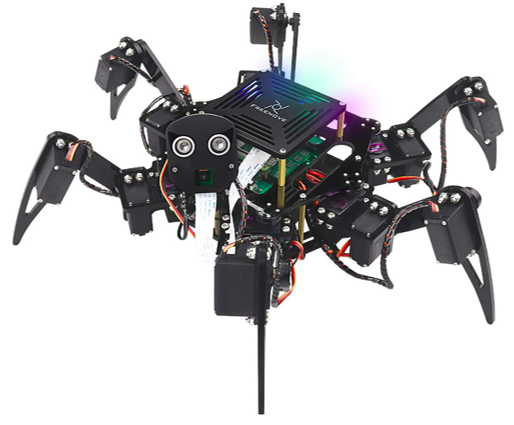
\includegraphics[scale=0.5]{figures/hexapod1.png}}
    \caption{The Freenove Big Hexapod robot kit}
    %\label{fig:Hexapod}
\end{figure}